\documentclass{report}
\usepackage{tikz}
\usepackage{amsmath}
\usepackage{amsthm}
\usepackage{amssymb}
\usepackage{bbold}
\usepackage{graphicx}

\graphicspath{{images/}}

\theoremstyle{definition}
\newtheorem{theorem}{Theorem}[chapter]
\newtheorem{corollary}[theorem]{Corollary}
\newtheorem{lemma}[theorem]{Lemma}
\newtheorem{problem}[theorem]{Problem}
\newtheorem{definition}[theorem]{Definition}

\newcommand{\R}{\mathbb{R}}
\newcommand{\N}{\mathbb{N}}
\renewcommand{\d}{\,\mathrm{d}}
\newcommand{\imat}{\mathbb{1}}
\newcommand{\zeromat}{\mathbb{0}}
\newcommand{\sprod}[2]{\left\langle #1 \middle| #2 \right\rangle}
\newcommand{\powerset}{\mathcal{P}}


\title{Bachelor thesis}
\author{Moritz Seppelt}
\date{\today}

\begin{document}


\maketitle

\tableofcontents

\chapter{Framework}
\section{Introduction}
\section{Graphs}
\begin{figure}[ht]
    \centering
    \begin{tikzpicture}[->,shorten >=1pt,auto,node distance=3cm,semithick]

    
      \node[circle, draw, fill=white, inner sep=2pt] (v1) {$v_1$};
      \node (v2) [below of=v1] {$v_2$};
      \node (v3) [right of=v2] {$v_3$};
      \node (v5) [right of=v1] {$v_5$};
      \node (v4) [right of=v5, below of=v5] {$v_4$};
    
      \path (v1) edge node {3} (v2)
            (v2) edge node {5} (v3)
            (v3) edge node {2} (v4)
            (v4) edge node {4} (v5)
            (v5) edge node {1} (v1)
            (v1) edge [loop left] node {6} (v1)
            (v3) edge node {7} (v5);
    \end{tikzpicture}
    \caption{Weighted Directed Graph with 5 Nodes}
\end{figure}

\begin{align*}
    A = \begin{bmatrix}
    \infty & 3 & \infty & \infty & \infty \\
    \infty & \infty & 5 & \infty & \infty \\
    \infty & \infty & \infty & 2 & 7 \\
    \infty & \infty & \infty & \infty & 4 \\
    1 & \infty & \infty & \infty & \infty \\
    \end{bmatrix}
\end{align*}
\section{The semiring}
\section{Einsums}
\subsection{Definition}
\subsection{Common examples}
\subsection{Properties}
\chapter{Shortest Path Problems}
\section{Introduction}
% Something about the importance of this problem family
\section{All pairs shortest path}
Here we see the power of exchanging the semiring for the first time. In this section we will use the tropical semiring $(\R \cup \{\infty\}, \min, +)$ and its induced matrix operations. But first we have to state the problem:
\begin{problem}[All pairs shortest path] 
    Given a directed weighted graph $G = (V, E)$ with $|V| = n$ and $|E| = m$ and its adjacency matrix $A$. Compute the length of the shortest path between every pair of nodes.
\end{problem}

\begin{lemma}
    Let $A \in \R^{n \times n}$ be an adjacency matrix. Then $(A^k)_{ij}$ holds the length of the shortest path with $k+1$ nodes between $v_i$ and $v_j$ for all $k \in \N$. 
\end{lemma}
\begin{proof}
    Let $D_k \in \R^{n \times n}$ ba a matrix such that $(D_k)_{ij}$ holds the length of the shortest path with $k+1$ nodes between $v_i$ and $v_j$. Thus we need to show that $A^k = D_k$ for all $k \in \N$ which we will do by induction. Namely, we need to show that (I) $D_0 = \imat_n$ and (II) $D_{k+1} = D_k \odot A$
    \begin{enumerate}
        \item[(I)] ...
        \item[(II)] ...
    \end{enumerate}
\end{proof}

\begin{lemma}
    Let $A \in \R^{n \times n}$ be an adjacency matrix of a directed weighted graph $G$. Then $G$ has no negative cycle $\Leftrightarrow$ 
    $$\sum_{k=0}^{n-1+q} A^k = \sum_{k=0}^{n-1} A^k \quad\forall q \in \N$$
\end{lemma}

\begin{corollary}
    A direct conclusion of the last lemma is that
    $$A^* = \sum_{k=0}^{\infty}A^k = \sum_{k=0}^{n-1}A^k$$
\end{corollary}

And $A^*$ solves our problem.

\subsection{Optimisiation in shortest path}
As we allready stated, shortest path only exist iff no negative cycles are present in the graph. This also means that if loop edges exist, their weight must be positive. Thus no shortest path will pass through these loops, because any path passing through these edges can be shortened by just removing this edge. So even if loops exist in the graph, they can be ignored for the shortest path calculations. We will modify the graph such that every vertex has a loop with weight 0, resulting in a new adjacency matrix $\tilde A$:
$$\tilde A_{ij} = \begin{cases}
    0  &\textrm{if}\quad i = j\\
    A_{ij} &\textrm{else}
\end{cases}$$
And it will hold that
$$A^* = \sum_{k=0}^{n-1}\tilde A^k$$

Using the next lemma we can simplify our computation:
\begin{lemma}
    Let $M, A \in \R^n$ with $\forall i \in [n]: A_{ii} = 0$. Using the matrix operation $\boxplus$ and $\boxdot$ induced by the tropical semiring we get that
    $$(M \boxdot A) \boxplus M = M \boxdot A$$ 
\end{lemma}
\begin{proof}
    \begin{align*}
        (M\boxdot A)_{ij} &= \min\{M_{i1} + A_{1j}, M_{i2} + A_{2j}, \dots, M_{in} + A_{nj}\}\\
        &\leq M_{ij} + A_{jj} = M_{ij} &&(*)\\
        ((M \boxdot A) \boxplus M)_{ij} &= \min\{(M\boxdot A)_{ij}, M_{ij}\} \stackrel{(*)}{=} (M\boxdot A)_{ij}
    \end{align*}
\end{proof}
Because $\tilde A$ has zeros on its diagonal we can apply this lemma, resulting in $\tilde A^{k+1} \boxplus \tilde A^k = \tilde A^{k+1}$ and thus the sum for computing $A^*$ collapses to the simple expression:
$$A^* = \tilde A^{n-1}$$

This result could also be achieved by looking at the problem from the graph theory perspective. $A^*_{ij}$ holds the length of shortest path between $v_i$ and $v_j$ of any number of edges less than $n$. But if every vertex has a loop with weight 0, every such path can be extended to a path with $n-1$ edges while preserving its length. So every shortest path with less than $n-1$ edges is a shortest path with $n-1$ edges und thus $A^* = \tilde A^{n-1}$.

\subsection{General Einsumisation of $A^*$}
To find a general expression in the language of Einsums we need to convert the sum of exponents in a sum of products. In this case we can actually boil it down to just one product. For this, we use this identity
$$\left(\begin{matrix}
    x & 1\\
    0 & 1
\end{matrix}\right)^k = \left(\begin{matrix}
    x^k & 1 + x + \dots + x^{k-1} \\
    0 & 1
\end{matrix}\right) \quad \forall k \in \N$$
which can be easily seen by induction. If we insert matricies instead of numbers in this two-by-two matrix and use the matrix operations induced by the semiring in use, we get
$$M(A) := \left(\begin{matrix}
    A & \imat\\
    \zeromat & \imat
\end{matrix}\right) \quad\Rightarrow\quad M(A)^n = \left(\begin{matrix}
    A^n & A^* \\
    \zeromat & \imat
\end{matrix}\right)$$
With this formulation, we can even drop the run-time form the previous $O(n^4)$ - $n$ matrix multiplications - to $O(n^3 \log n)$, because we can compute the $n$-th power of a matrix using $O(\log n)$ matrix multiplications. Using the Strassen-Algorithm for matrix multiplication we can even get down to $O(n^{\log_27}\log n)$.

The corresponding Einsum string is just the representation of matrix exponentiation:
$$it_1,t_1t_2,\dots, t_{n-2}t_{n-1},t_{n-1}j \rightarrow ij, M(A)$$

\subsection{Old derivation}
Our goal was more ambitious than just solving the problem. We wanted to state the solution in the language of Einsums. For that we need to go up one dimension. Let $R_{ijk} := A^{n-1}_{ij}$ be a tensor. Now we can rewrite $A^*$ as follows
$$A^*_{ij} = \sum_{k=0}^{n-1} A^k_{ij} = \sum_{k=1}^{n}A^{k-1}_{ij} = \sum_{k=1}^{n}R_{ijk}$$
This expression is allready in the necessary shape. The last step is to compute $R_{ijk}$. For that we need to define even more tensors: 
$$A^{(l)}_{ijk} := 
\begin{cases}
    A_{ij} & \textrm{if}\quad l \leq k\\
    \imat_{ij} & \textrm{else}   
\end{cases}
$$
As shown in Fig. \ref*{fig:shortest_path_tensor} we just need to multiply all matricies at each level together and than add the result up.

\begin{figure}[h]
    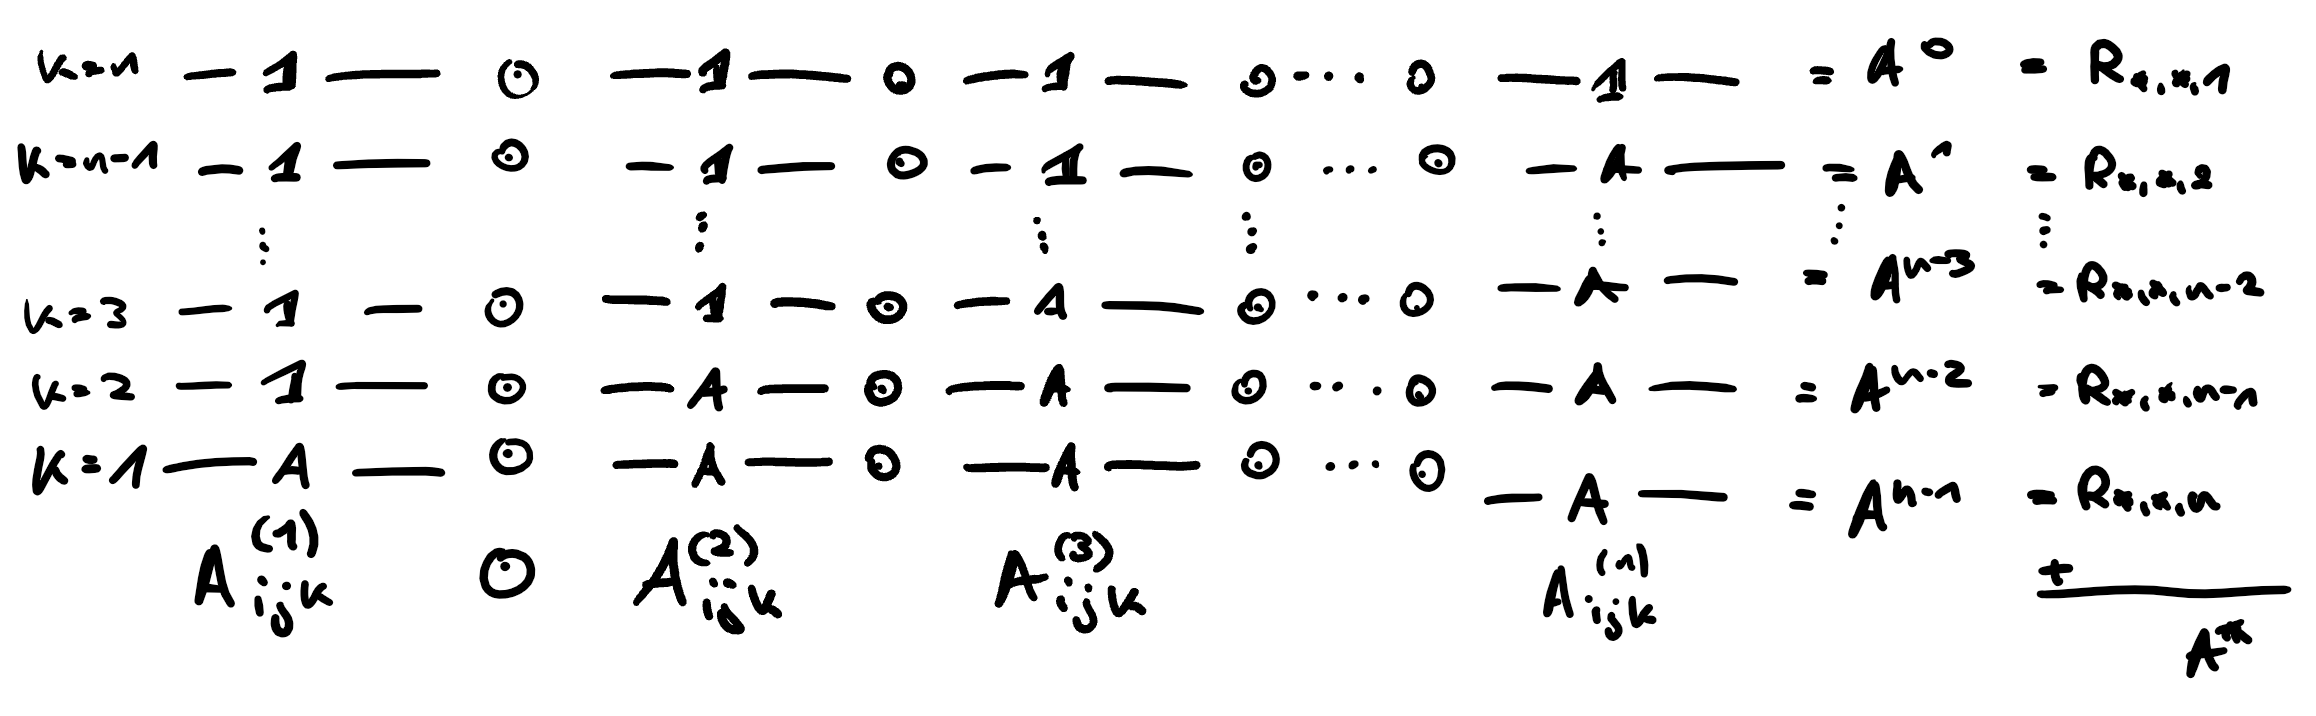
\includegraphics[width=\linewidth]{shortest_path_tensor.png}
    \caption{Visualized the shortest path tensors}
    \label{fig:shortest_path_tensor}
\end{figure}

The resulting expression comes out to be
$$A^*_{ij} = \sum_{k, t_1, \dots, t_{n-1} \in [n]} A^{(1)}_{it_1k}A^{(2)}_{t_1t_2k}A^{(3)}_{t_2t_3k}\dots A^{(n-1)}_{t_{n-2}t_{n-1}k}A^{(n)}_{t_{n-1}jk}$$
Which correspond to the Einsum string
$$it_1k, t_1t_2k, t_2t_3k, \cdots, t_{n-2}t_{n-1}k, t_{n-1}jk \to ij$$

\section{All pairs longest path}
The computation is exactly the same as in the All pairs shortest path problem. The only difference is the semiring in use. Here we need $(\R \cup \{-\infty\}, \max, +)$ and there must not exist a positive cycle. Then just compute $A^*$ and the entry $A^*_{ij}$ holds the longest path from $v_i$ to $v_j$. [Small note on convergency of $A^*$]

\section{Minimum weight spanning tree}
Here we need the observation that the edge $(v, u)$ is not included in the MST iff its weight is larger than the maximum weight of any path between $v$ and $u$. [Add proof] This we can model, by defining the weight of a path as the maximum of the weights of its edges. Then we compute the all pairs shortest path problem, but now we have exchanged the $+$-operation by the $\max$-operation, which means we have to use the $(\R \cup\{\infty\}, \min, \max)$ semiring. After computing $A^*$ we include the edge $(v_i, v_j)$ in the minimum weight spanning tree iff $A_{ij} \leq A^*_{ij}$.
[Diskuss conergency of $A^*$]

\section{Further Problems}
\begin{itemize}
    \item Marko Chaines. Using the semiring $([0, 1], +, \cdot)$ $A^k_{ij}$ holds the propability that an agent reaches $v_j$ starting at $v_i$ after $k$ steps if the weights of the edges symbolze the properbility that an agent moves along this edge.
    \item Reachability / Transitive hull. In an undirected unweighted graph, we ask the question whether a vertex $v_j$ is reachable starting at vertex $v_i$. For that we could just compute the shortest path and see whether $A^*_{ij}$ is infinite or not. But we can achieve the same with less information by just using the $(\{0, 1\}, \lor, \land)$ semiring and check whether $A^*_{ij} = 1$.
\end{itemize}



\end{document}